% ===========================================================================
% EARLIER DRAFT of the roofline section (pre-revision), kept verbatim.
% Superseded by roofline.tex; \input at the end of that file under a
% "speculative" banner. Uses the old F, S, C, I^mem, I^net, rho notation and
% references the removed factors table (tab:roofline-factors -> "??").
% ===========================================================================
\medskip
\noindent\fbox{\parbox{\dimexpr\linewidth-2\fboxsep-2\fboxrule}{\color{red}\small
\textbf{Speculative / earlier draft, not revised.} Everything from here to the end of the
section is the earlier version of this model, kept for reference. It uses the old per-node
quantities ($F$, $S$, $C$, $I^{\mathrm{mem}}$, $I^{\mathrm{net}}$, $\rho$), peak rather than
measured rates, and refers to a per-model factors table that has been removed (those
references print as ``??''). Table~\ref{tab:roofline-validation} was generated with this
earlier model.}}
\medskip

\subsection*{Earlier draft (speculative)}

{\color{red}[TODO: I don't see much value in the subsection below. Come back to it if it is useful.]}
\subsection{Notation}
\label{sec:roofline-notation}

\begin{table}[h]
\centering
\caption{Symbols. Per layer, a block has $|V|$ destination nodes and $|E|$ sampled edges;
all per-node quantities are block totals divided by $|V|$.}
\label{tab:roofline-notation}
\small
\begin{tabular}{l p{7.6cm} p{4.6cm}}
\toprule
Symbol & Meaning & Typical value \\
\midrule
$h$ & hidden width (feature row length) & $256$--$4096$ \\
$b$ & bytes per value (fp32) & $4$ \\
$f$ & fanout $=$ sampled in-degree per destination node ($|E| = f|V|$) & $15$ \\
$H$ & GAT heads & $4$ \\
$\rho$ & frontier expansion $|V_{\mathrm{src}}|/|V|$ of a block ($1<\rho\le f{+}1$) & $\approx 6$ \\
$r$ & remote source rows per destination node (shuffle volume) & measured \\
$\delta$ & data-parallel redundancy: nodes computed $\div$ unique nodes ($\ge 1$) & measured \\
\midrule
$P$ & dense (GEMM) peak rate & $19.5$\,TFLOP/s (A100 fp32) \\
$B_{\mathrm{mem}}$ & GPU DRAM bandwidth & $2.0$\,TB/s (A100-80GB) \\
$B_{\mathrm{net}}$ & effective per-GPU all-to-all (shuffle) bandwidth & $\approx 1$\,GB/s PCIe-emu; $\approx 54$\,GB/s NVLink \\
\midrule
$F$ & dense FLOPs per node per layer (fwd$+$bwd) & model-dependent \\
$S$ & DRAM bytes per node per layer (sparse gathers $+$ GEMM operands) & model-dependent \\
$C$ & interconnect bytes to pull one node (row in, gradient out) & $2hb$ \\
\bottomrule
\end{tabular}
\end{table}


\paraq{What do the factors say before any hardware number is plugged in?}
Three things. (i)~Both models cross the memory ridge ($\approx 10$\,FLOP/B) already at
$h\approx 150$, so from $h=256$ up the per-node compute is GEMM-bound \emph{at peak}; below
that, and in practice for small kernels, it is bandwidth/latency bound. (ii)~The network
intensity grows linearly in $h$ while the shuffle cost per node grows only linearly in $h$ and
the dense work quadratically: \textbf{a wider layer is, per node, more compute-bound, not more
communication-bound}. (iii)~For SAGE $I^{\mathrm{net}}$ does not depend on the node's degree,
so all remote nodes of a layer fall on the same side of the ridge; for GAT it scales with the
node's source count, so the remote nodes of a layer are \emph{spread} and the vote of
Section~\ref{sec:roofline-algo} is a genuine distribution.

% AUTO-GENERATED by gen_roofline.py -- edit the script, not this file.
\begin{table}[h]
\centering
\caption{Roofline demands and bounds per destination node per layer (forward$+$backward, fp32, fanout $f{=}15$, GAT $H{=}4$, $\rho{=}6$). $T^{\mathrm{cmp}}=F/P+S/B_{\mathrm{mem}}$ at A100 peak ($P{=}19.5$\,TFLOP/s, $B_{\mathrm{mem}}{=}2.0$\,TB/s); $T^{\mathrm{net}}=C/B_{\mathrm{net}}$ with effective $B_{\mathrm{net}}$ of PCIe-emu 1\,GB/s, NVLink 54\,GB/s.}
\label{tab:roofline-instances}
\footnotesize\setlength{\tabcolsep}{3.5pt}
\resizebox{\linewidth}{!}{%
\begin{tabular}{l r | r r r | r r | r r | r r}
\toprule
Model & $h$ & $F$ & $S$ & $C$ & $I^{\mathrm{mem}}$ & $I^{\mathrm{net}}$ & $T^{\mathrm{cmp}}$ & $P_{\mathrm{eff}}$ & $T^{\mathrm{net}}_{\text{PCIe-emu}}$ & $T^{\mathrm{net}}_{\text{NVLink}}$ \\
 & & (FLOP) & (B) & (B) & (FLOP/B) & (FLOP/B) & & (TFLOP/s) & (ratio to $T^{\mathrm{cmp}}$) & (ratio to $T^{\mathrm{cmp}}$) \\
\midrule
SAGE & 256 & 786\,kFLOP & 43\,kB & 2.05\,kB & 18 & 384 & 62\,ns & 12.7 & 2.05\,\si{\micro\second} (33$\times$) & 38\,ns (0.61$\times$) \\
SAGE & 1024 & 12.6\,MFLOP & 172\,kB & 8.19\,kB & 73 & 1536 & 731\,ns & 17.2 & 8.19\,\si{\micro\second} (11$\times$) & 152\,ns (0.21$\times$) \\
SAGE & 4096 & 201\,MFLOP & 688\,kB & 32.8\,kB & 293 & 6144 & 10.67\,\si{\micro\second} & 18.9 & 32.77\,\si{\micro\second} (3.1$\times$) & 607\,ns (0.057$\times$) \\
\midrule
GAT & 256 & 2.36\,MFLOP & 101\,kB & 2.05\,kB & 23 & 1152 & 171\,ns & 13.8 & 2.05\,\si{\micro\second} (12$\times$) & 38\,ns (0.22$\times$) \\
GAT & 1024 & 37.7\,MFLOP & 396\,kB & 8.19\,kB & 95 & 4608 & 2.13\,\si{\micro\second} & 17.7 & 8.19\,\si{\micro\second} (3.8$\times$) & 152\,ns (0.071$\times$) \\
GAT & 4096 & 604\,MFLOP & 1.58\,MB & 32.8\,kB & 383 & 18432 & 31.76\,\si{\micro\second} & 19.0 & 32.77\,\si{\micro\second} (1$\times$) & 607\,ns (0.019$\times$) \\
\bottomrule
\end{tabular}}
\end{table}


% ---------------------------------------------------------------------------
\subsection{Adding the interconnect: the nested roofline}
\label{sec:roofline-net}

\paraq{What does pulling a node cost, and when is it cheaper than recomputing it?}
Pulling a node's hidden state moves one $h$-wide row in the forward pass and one gradient row
back, $C = 2hb$ bytes, at the effective all-to-all rate:
\begin{equation}
  T^{\mathrm{net}} = \frac{C}{B_{\mathrm{net}}}, \qquad
  I^{\mathrm{net}} = \frac{F}{C}.
  \label{eq:Tnet}
\end{equation}
The node is \textbf{compute-bound} when its compute time exceeds its transfer time, i.e.\ when
its network intensity lies to the right of the network ridge:
\begin{equation}
  \boxed{\;
  T^{\mathrm{cmp}} > T^{\mathrm{net}}
  \;\Longleftrightarrow\;
  I^{\mathrm{net}} > \frac{P_{\mathrm{eff}}}{B_{\mathrm{net}}}
  \;\Longrightarrow\; \text{pull (split)};\qquad
  \text{otherwise recompute (data parallel).}
  \;}
  \label{eq:ridge}
\end{equation}
Written as a single attainable rate, the node sits under three roofs at once:
\begin{equation}
  \text{rate} = \min\!\big(\, P,\;\; B_{\mathrm{mem}}\, I^{\mathrm{mem}},\;\; B_{\mathrm{net}}\, I^{\mathrm{net}} \,\big),
  \label{eq:nested}
\end{equation}
which is the nested roofline of Figure~\ref{fig:roofline}: the inner (memory) roofline lowers
the dense roof to $P_{\mathrm{eff}}$, and the outer (network) roofline places the node as
compute- or communication-bound. Unlike a classical roofline the node therefore has two
intensities, $I^{\mathrm{mem}}$ and $I^{\mathrm{net}}$.

\begin{figure}[h]
  \centering
  % AUTO-GENERATED by gen_roofline.py -- edit the script, not this file.
% Standalone tikzpicture: \input it in the thesis or a beamer slide
% (needs \usepackage{pgfplots} \pgfplotsset{compat=1.18}).
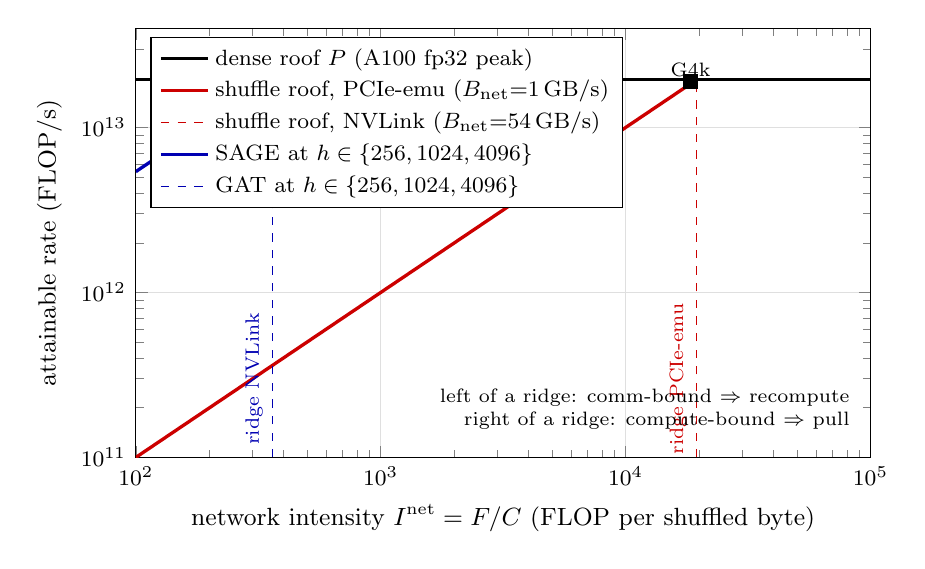
\begin{tikzpicture}
\begin{loglogaxis}[
  width=0.9\linewidth, height=0.58\linewidth,
  xmin=100, xmax=100000, ymin=1e+11, ymax=4e+13,
  xlabel={network intensity $I^{\mathrm{net}} = F/C$ (FLOP per shuffled byte)},
  ylabel={attainable rate (FLOP/s)},
  grid=major, grid style={gray!25},
  legend style={at={(0.02,0.98)}, anchor=north west, font=\footnotesize, cells={anchor=west}},
  tick label style={font=\footnotesize}, label style={font=\small},
]
\addplot[very thick, black] coordinates {(100,1.95e+13) (100000,1.95e+13)};
\addlegendentry{dense roof $P$ (A100 fp32 peak)}
\addplot[very thick, red!80!black] coordinates {(100,1e+11) (19500,1.95e+13)};
\addlegendentry{shuffle roof, PCIe-emu ($B_{\mathrm{net}}{=}1$\,GB/s)}
\addplot[dashed, red!80!black, thin] coordinates {(19500,1e+11) (19500,1.95e+13)};
\node[red!80!black, font=\scriptsize, anchor=south, rotate=90] at (axis cs:19500,3e+11) {ridge PCIe-emu};
\addplot[very thick, blue!70!black] coordinates {(100,5.4e+12) (361.111,1.95e+13)};
\addlegendentry{shuffle roof, NVLink ($B_{\mathrm{net}}{=}54$\,GB/s)}
\addplot[dashed, blue!70!black, thin] coordinates {(361.111,1e+11) (361.111,1.95e+13)};
\node[blue!70!black, font=\scriptsize, anchor=south, rotate=90] at (axis cs:361.111,3e+11) {ridge NVLink};
\addplot[only marks, mark=*, mark size=2.6pt, black] coordinates {(384,1.27185e+13) (1536,1.72064e+13) (6144,1.88711e+13)};
\addlegendentry{SAGE at $h\in\{256,1024,4096\}$}
\node[font=\scriptsize, anchor=north, inner sep=1.5pt] at (axis cs:384,1.27185e+13) {S256};
\node[font=\scriptsize, anchor=north, inner sep=1.5pt] at (axis cs:1536,1.72064e+13) {S1k};
\node[font=\scriptsize, anchor=north, inner sep=1.5pt] at (axis cs:6144,1.88711e+13) {S4k};
\addplot[only marks, mark=square*, mark size=2.6pt, black] coordinates {(1152,1.37696e+13) (4608,1.76922e+13) (18432,1.90164e+13)};
\addlegendentry{GAT at $h\in\{256,1024,4096\}$}
\node[font=\scriptsize, anchor=south, inner sep=1.5pt] at (axis cs:1152,1.37696e+13) {G256};
\node[font=\scriptsize, anchor=south, inner sep=1.5pt] at (axis cs:4608,1.76922e+13) {G1k};
\node[font=\scriptsize, anchor=south, inner sep=1.5pt] at (axis cs:18432,1.90164e+13) {G4k};
\node[font=\scriptsize, anchor=south east, align=right] at (axis cs:90000,1.3e+11) {left of a ridge: comm-bound $\Rightarrow$ recompute\\right of a ridge: compute-bound $\Rightarrow$ pull};
\end{loglogaxis}
\end{tikzpicture}

  \caption{\textbf{Nested roofline} (log--log). Black: dense roof $P$. Coloured: shuffle
  roofs $B_{\mathrm{net}} I^{\mathrm{net}}$ for emulated PCIe and NVLink, with their ridges
  $P/B_{\mathrm{net}}$ dashed. Markers: SAGE ($\bullet$) and GAT ($\blacksquare$) at
  $h\in\{256,1024,4096\}$, plotted at their network intensity and their memory-lowered
  compute roof $P_{\mathrm{eff}}$ (Table~\ref{tab:roofline-instances}). A marker left of a
  ridge is communication-bound on that interconnect (recompute wins); right of it,
  compute-bound (pull wins).}
  \label{fig:roofline}
\end{figure}

\paraq{Where are things expected to fall?}
With the preliminary rates of Table~\ref{tab:roofline-notation} the ridges sit at
$\approx 2\times10^{4}$\,FLOP/B (PCIe-emu) and $\approx 3.6\times10^{2}$\,FLOP/B (NVLink).
\expected{On emulated PCIe every SAGE and GAT point up to $h{=}4096$ is communication-bound
(SAGE by $33\times$, $11\times$, $3\times$ at $h=256,1024,4096$; GAT by $12\times$, $4\times$,
$1\times$), so recomputation (data parallelism) is predicted for the remote nodes, with GAT at
$h{=}4096$ exactly on the ridge. On NVLink every point except SAGE $h{=}256$ (at $0.6\times$,
near the ridge) is compute-bound, so pulling (split) is predicted.} Because
$I^{\mathrm{net}}\propto h$, the predicted ordering along the hidden-size ladder is that
\emph{wider} layers move toward split, not away from it; GAT, with $\rho$ times more dense
work per pulled byte, reaches the ridge at roughly $\rho/2 \approx 3\times$ smaller $h$ than
SAGE.

% ---------------------------------------------------------------------------
\subsection{From one node to a strategy per layer}
\label{sec:roofline-strategy}

\paraq{How do the per-node costs compose into the cost of each strategy?}
Let $V_\ell$ be the unique nodes of layer $\ell$, $R_\ell$ the remote (node, requesting-GPU)
pairs that split would shuffle ($|R_\ell| = r_\ell |V_\ell|$), and $D_\ell$ the extra
(node, GPU) pairs data parallelism would compute redundantly
($|D_\ell| = (\delta_\ell - 1)|V_\ell|$). Then, per layer,
\begin{align}
  T^{\mathrm{split}}_\ell &= \sum_{v\in V_\ell} T^{\mathrm{cmp}}_v + \sum_{(u,g)\in R_\ell} T^{\mathrm{net}}_u, \label{eq:split}\\
  T^{\mathrm{dp}}_\ell    &= \sum_{v\in V_\ell} T^{\mathrm{cmp}}_v + \sum_{(u,g)\in D_\ell} T^{\mathrm{cmp}}_u, \label{eq:dp}\\
  T^{\mathrm{pipe}}_\ell  &= \max\!\Big(\sum_{v\in V_\ell} T^{\mathrm{cmp}}_v,\; \sum_{(u,g)\in R_\ell} T^{\mathrm{net}}_u\Big)
                             + (1-\eta)\min(\cdot,\cdot), \label{eq:pipe}
\end{align}
where $\eta\in[0,1]$ is the overlap efficiency of the pipeline hybrid on the given machine
($\eta{=}1$: perfect overlap; $\eta{=}0$: none). The first sums are common to all
three; the decision is between the \emph{redundant} terms:
\begin{equation}
  \text{data parallel at } \ell \iff
  \sum_{(u,g)\in D_\ell} T^{\mathrm{cmp}}_u \;<\; \sum_{(u,g)\in R_\ell} T^{\mathrm{net}}_u .
  \label{eq:layer-decision}
\end{equation}
When $D_\ell$ and $R_\ell$ are the same node set (one GPU needs one remote node once), this
is exactly the per-node test \eqref{eq:ridge} applied to every remote node and summed---the
cost-weighted majority vote. The pipeline hybrid is worth enabling at a split layer only near
the ridge: its saving over \eqref{eq:split} is $\eta\min(T^{\mathrm{cmp}},T^{\mathrm{net}})$,
largest when the two are balanced and vanishing when either dominates; we therefore enable it
when $1/\beta \le T^{\mathrm{net}}_\ell/T^{\mathrm{cmp}}_\ell \le \beta$ for a tunable
$\beta$ (\expected{$\beta\approx 3$}).

% ---------------------------------------------------------------------------
\subsection{The approximate algorithm}
\label{sec:roofline-algo}

\paraq{What is the procedure, end to end?}
The expensive inputs---which nodes are remote, which are redundant, and their degrees---come
from \emph{sampling alone}: one pass of the sampler per strategy variant, without features,
training, or multiple GPUs. Everything else is arithmetic.

\begin{algorithm}[h]
\caption{Roofline-guided choice of the per-layer strategy}
\label{alg:roofline}
\begin{algorithmic}[1]
\Require graph, partition map, model $\in\{\text{SAGE},\text{GAT}\}$, depth $L$, width $h$,
         fanout $f$, heads $H$; hardware rates $P, B_{\mathrm{mem}}, B_{\mathrm{net}}$;
         overlap efficiency $\eta$, band $\beta$
\State \textbf{Sample the split variant:} for each hop $\ell$ record the remote pairs
       $R_\ell$ and each node's sampled degree $d_u$ \Comment{gives $r_\ell$}
\State \textbf{Sample the data-parallel variant:} per-GPU micro-batch trees; for each hop
       $\ell$ record the redundant pairs $D_\ell$ and degrees \Comment{gives $\delta_\ell$}
\For{each hop $\ell = 0,\dots,L-1$ (seeds outward)}
  \For{each remote node $u \in R_\ell \cup D_\ell$}
    \State $F_u, S_u \gets$ Table~\ref{tab:roofline-factors} with $d_u$ in place of $f$
           (and $\rho$ for GAT); $C_u \gets 2hb$
    \State $T^{\mathrm{cmp}}_u \gets F_u/P + S_u/B_{\mathrm{mem}}$;\quad
           $T^{\mathrm{net}}_u \gets C_u/B_{\mathrm{net}}$
    \State label $u$ \textsc{pull} if $T^{\mathrm{cmp}}_u > T^{\mathrm{net}}_u$ else \textsc{recompute}
           \Comment{Eq.~\eqref{eq:ridge}}
  \EndFor
  \State $\mathrm{vote}_\ell \gets$ majority label over $R_\ell$ (cost-weighted: Eq.~\eqref{eq:layer-decision})
  \State $T^{\mathrm{split}}_\ell, T^{\mathrm{dp}}_\ell, T^{\mathrm{pipe}}_\ell \gets$ Eqs.~\eqref{eq:split}--\eqref{eq:pipe}
\EndFor
\State \textbf{Prefix constraint:} data-parallel hops must be contiguous from the seeds, so
       $k^\star \gets \arg\min_k \big[\sum_{\ell<k} T^{\mathrm{dp}}_\ell + \sum_{\ell\ge k} T^{\mathrm{split}}_\ell\big]$
       \Comment{equals the first hop whose vote flips to \textsc{pull} when votes are monotone}
\State \textbf{Pipeline:} at each split hop $\ell\ge k^\star$ enable overlap iff
       $1/\beta \le T^{\mathrm{net}}_\ell / T^{\mathrm{cmp}}_\ell \le \beta$
\State \Return $k^\star$, overlap flags, and the predicted epoch time
       $T^{\mathrm{fixed}} + \sum_\ell T_\ell$ \Comment{$T^{\mathrm{fixed}}$: sampling $+$ input-feature load}
\end{algorithmic}
\end{algorithm}

% ---------------------------------------------------------------------------
\subsection{Scope of the model}
\label{sec:roofline-scope}

\paraq{What is modelled analytically and what is taken from measurement?}
The roofline is first-order by design: it prices every node from three hardware rates and the
factors of Table~\ref{tab:roofline-factors}. Two quantities are folded into measured
constants rather than modelled: the per-epoch fixed term $T^{\mathrm{fixed}}$ (sampling and
input-feature loading, independent of $h$) and the overlap efficiency $\eta$. The fixed term
also explains an epoch-level effect the per-node ratio alone would hide: because
$T^{\mathrm{fixed}}$ does not grow with $h$, the shuffle's \emph{share} of an epoch rises along
the hidden-size ladder even as the per-node ratio $T^{\mathrm{net}}/T^{\mathrm{cmp}}\propto 1/h$
falls. \expected{Along the hidden-size ladder the training-only gap between split and data
parallel stops widening at the largest $h$.}

% ---------------------------------------------------------------------------
\subsection{Validation: predicted versus measured winner}
\label{sec:roofline-validation}

\paraq{What must a decision model get right?}
Not the epoch time to within a tolerance, but the \emph{winner}. The check is therefore
per cell: the roofline's verdict for that (model, $h$, interconnect) against the measured
winner of the training-only time, which is the quantity the model prices
(Table~\ref{tab:roofline-validation}). The per-epoch winner is listed beside it; where the
two differ, the difference is the $h$-independent fixed term of
Section~\ref{sec:roofline-scope}.

% AUTO-GENERATED by gen_roofline_validation.py -- edit the script, not this file.
\begin{table}[h]
\centering
\caption{Decision check with the \emph{current} (peak-rate) constants: the roofline's per-layer verdict---pull (split) if $T^{\mathrm{cmp}}>T^{\mathrm{net}}$, else recompute (DGL/data parallel)---against the measured winner per cell (4$\times$A100, no feature cache, mean over runs). Train $=$ forward$+$backward, the quantity the roofline prices; epoch $=$ per-epoch duration for reference. $T^{\mathrm{net}}/T^{\mathrm{cmp}}$ is the model's ratio for that (model, $h$, interconnect). \checkmark{} $=$ prediction matches the train-only winner.}
\label{tab:roofline-validation}
\footnotesize\setlength{\tabcolsep}{4pt}
\resizebox{\linewidth}{!}{%
\begin{tabular}{l l l r r | r r | r r | l l | c l}
\toprule
graph & hw & model & $L$ & $h$ & split train & DGL train & split epoch & DGL epoch & win (train) & win (epoch) & pred & $T^{\mathrm{net}}/T^{\mathrm{cmp}}$ \\
\midrule
papers100M & NVLink & gat & 2 & 1024 & 9.6 & 7.8 & 13.6 & 11.3 & dgl & dgl & $\times$ split & 0.071 \\
papers100M & NVLink & gat & 3 & 256 & 13.5 & 12.6 & 21.2 & 19.4 & dgl & dgl & $\times$ split & 0.22 \\
papers100M & NVLink & gat & 3 & 1024 & 22.9 & 28.1 & 29.8 & 35.2 & split & split & \checkmark split & 0.071 \\
papers100M & NVLink & gat & 3 & 4096 & 138.0 & 190.2 & 146.1 & 197.7 & split & split & \checkmark split & 0.019 \\
papers100M & NVLink & gat & 4 & 1024 & 80.6 & 114.3 & 97.6 & 134.7 & split & split & \checkmark split & 0.071 \\
papers100M & NVLink & sage & 2 & 1024 & 3.8 & 3.1 & 7.6 & 6.7 & dgl & dgl & $\times$ split & 0.21 \\
papers100M & NVLink & sage & 3 & 256 & 5.5 & 5.1 & 12.9 & 11.7 & dgl & dgl & $\times$ split & 0.61 \\
papers100M & NVLink & sage & 3 & 1024 & 8.3 & 7.5 & 15.7 & 14.2 & dgl & dgl & $\times$ split & 0.21 \\
papers100M & NVLink & sage & 3 & 4096 & 49.8 & 54.0 & 58.6 & 61.2 & split & split & \checkmark split & 0.057 \\
papers100M & NVLink & sage & 4 & 256 & 11.7 & 9.5 & 28.0 & 28.9 & dgl & split & $\times$ split & 0.61 \\
papers100M & NVLink & sage & 4 & 1024 & 31.4 & 38.2 & 48.4 & 57.9 & split & split & \checkmark split & 0.21 \\
\midrule
papers100M & PCIe-emu & gat & 2 & 1024 & 9.0 & 7.9 & 12.6 & 11.3 & dgl & dgl & \checkmark dgl & 3.8 \\
papers100M & PCIe-emu & gat & 3 & 256 & 15.4 & 13.0 & 22.9 & 19.7 & dgl & dgl & \checkmark dgl & 12 \\
papers100M & PCIe-emu & gat & 3 & 1024 & 26.9 & 28.8 & 33.6 & 35.9 & split & split & $\times$ dgl & 3.8 \\
papers100M & PCIe-emu & gat & 3 & 4096 & 149.8 & 190.4 & 157.5 & 197.9 & split & split & $\times$ dgl & 1 \\
papers100M & PCIe-emu & gat & 4 & 1024 & 97.9 & 115.3 & 114.8 & 135.8 & split & split & $\times$ dgl & 3.8 \\
papers100M & PCIe-emu & sage & 2 & 1024 & 4.1 & 3.3 & 7.7 & 6.8 & dgl & dgl & \checkmark dgl & 11 \\
papers100M & PCIe-emu & sage & 3 & 256 & 6.0 & 5.4 & 13.0 & 12.5 & dgl & dgl & \checkmark dgl & 33 \\
papers100M & PCIe-emu & sage & 3 & 1024 & 12.3 & 8.3 & 19.3 & 15.0 & dgl & dgl & \checkmark dgl & 11 \\
papers100M & PCIe-emu & sage & 3 & 4096 & 64.1 & 60.3 & 72.7 & 67.5 & dgl & dgl & \checkmark dgl & 3.1 \\
papers100M & PCIe-emu & sage & 4 & 256 & 20.5 & 11.0 & 37.1 & 30.9 & dgl & dgl & \checkmark dgl & 33 \\
papers100M & PCIe-emu & sage & 4 & 1024 & 50.5 & 40.0 & 67.7 & 59.8 & dgl & dgl & \checkmark dgl & 11 \\
\midrule
products & NVLink & gat & 2 & 1024 & 2.1 & 1.9 & 3.3 & 2.5 & dgl & dgl & $\times$ split & 0.071 \\
products & NVLink & gat & 3 & 256 & 3.6 & 3.9 & 6.4 & 6.2 & split & dgl & \checkmark split & 0.22 \\
products & NVLink & gat & 3 & 1024 & 11.0 & 13.3 & 13.9 & 15.5 & split & split & \checkmark split & 0.071 \\
products & NVLink & gat & 3 & 4096 & 75.8 & 88.5 & 78.8 & 90.8 & split & split & \checkmark split & 0.019 \\
products & NVLink & gat & 4 & 256 & 11.2 & 15.1 & 17.5 & 23.4 & split & split & \checkmark split & 0.22 \\
products & NVLink & gat & 4 & 1024 & 50.7 & 71.6 & 57.2 & 79.5 & split & split & \checkmark split & 0.071 \\
products & NVLink & sage & 2 & 1024 & 0.8 & 0.6 & 2.0 & 1.3 & dgl & dgl & $\times$ split & 0.21 \\
products & NVLink & sage & 3 & 256 & 1.3 & 1.1 & 4.2 & 3.5 & dgl & dgl & $\times$ split & 0.61 \\
products & NVLink & sage & 3 & 1024 & 2.6 & 2.5 & 5.5 & 4.8 & dgl & dgl & $\times$ split & 0.21 \\
products & NVLink & sage & 3 & 4096 & 14.7 & 14.3 & 18.0 & 16.7 & dgl & dgl & $\times$ split & 0.057 \\
products & NVLink & sage & 4 & 256 & 4.7 & 4.8 & 11.0 & 13.2 & split & split & \checkmark split & 0.61 \\
products & NVLink & sage & 4 & 1024 & 16.1 & 17.9 & 22.8 & 26.0 & split & split & \checkmark split & 0.21 \\
products & NVLink & sage & 4 & 4096 & 140.4 & 155.1 & 147.2 & 163.4 & split & split & \checkmark split & 0.057 \\
products & NVLink & sage & 6 & 1024 & 163.3 & 332.4 & 177.5 & 364.8 & split & split & \checkmark split & 0.21 \\
\midrule
products & PCIe-emu & gat & 2 & 1024 & 2.3 & 1.9 & 3.1 & 2.6 & dgl & dgl & \checkmark dgl & 3.8 \\
products & PCIe-emu & gat & 3 & 256 & 4.6 & 3.9 & 7.1 & 6.2 & dgl & dgl & \checkmark dgl & 12 \\
products & PCIe-emu & gat & 3 & 1024 & 13.1 & 13.0 & 15.6 & 15.2 & dgl & dgl & \checkmark dgl & 3.8 \\
products & PCIe-emu & gat & 3 & 4096 & 82.5 & 88.7 & 85.1 & 91.0 & split & split & $\times$ dgl & 1 \\
products & PCIe-emu & gat & 4 & 256 & 16.0 & 15.1 & 22.0 & 23.3 & dgl & split & \checkmark dgl & 12 \\
products & PCIe-emu & gat & 4 & 1024 & 63.7 & 71.6 & 70.1 & 79.5 & split & split & $\times$ dgl & 3.8 \\
products & PCIe-emu & sage & 2 & 1024 & 0.8 & 0.6 & 1.6 & 1.4 & dgl & dgl & \checkmark dgl & 11 \\
products & PCIe-emu & sage & 3 & 256 & 2.2 & 1.1 & 4.8 & 3.5 & dgl & dgl & \checkmark dgl & 33 \\
products & PCIe-emu & sage & 3 & 1024 & 4.6 & 2.6 & 7.2 & 4.8 & dgl & dgl & \checkmark dgl & 11 \\
products & PCIe-emu & sage & 3 & 4096 & 21.3 & 14.1 & 24.1 & 16.5 & dgl & dgl & \checkmark dgl & 3.1 \\
products & PCIe-emu & sage & 4 & 256 & 9.5 & 4.8 & 15.5 & 13.2 & dgl & dgl & \checkmark dgl & 33 \\
products & PCIe-emu & sage & 4 & 1024 & 29.5 & 18.1 & 36.0 & 26.1 & dgl & dgl & \checkmark dgl & 11 \\
products & PCIe-emu & sage & 4 & 4096 & 196.1 & 154.0 & 202.7 & 162.3 & dgl & dgl & \checkmark dgl & 3.1 \\
products & PCIe-emu & sage & 6 & 1024 & 246.7 & 331.2 & 260.8 & 363.7 & split & split & $\times$ dgl & 11 \\
\midrule
\multicolumn{13}{l}{agreement with the train-only winner: 33/50 cells (NVLink 14/25; PCIe-emu 19/25)} \\
\bottomrule
\end{tabular}}
\end{table}


% ===========================================================================
% DRAFT REVIEW BOX -- for the author's pass; remove before submission.
% ===========================================================================
\noindent\rule{\linewidth}{0.8pt}
{\footnotesize
\noindent\textbf{\color{red}Draft review notes (remove before submission).} Points from the
2026-11-03 review of this section, in order of priority, with the concerns they answer.
\begin{enumerate}\itemsep2pt
  \item \textbf{Use achieved rates, not peak (``measured roofline'').} Measure one layer's GEMM rate
        and gather bandwidth at the target $h$ on one GPU and use those for $P$ and
        $B_{\mathrm{mem}}$ in Table~\ref{tab:roofline-instances} and Figure~\ref{fig:roofline}.
        \emph{Concern:} at $h\le 1024$ the measured per-layer time is roughly \emph{linear} in $h$,
        not quadratic---the GEMMs are far below $19.5$\,TFLOP/s---so the peak-rate dense roof is
        decorative there and the memory roof is the operative one. This is also the source of the
        direction tension below.
  \item \textbf{Measure $B_{\mathrm{net}}$ directly} (4-GPU NCCL all-to-all microbenchmark) and
        replace the subtraction-derived $\approx 1$ / $\approx 54$\,GB/s. \emph{Concern:} the PCIe-emu
        ridge moves 1:1 with this constant; it is the easiest question to be asked.
  \item \textbf{Pitch: the roofline supplies unit costs, sampling supplies counts.} The per-layer
        decision is $\delta_\ell\,T^{\mathrm{cmp}}$ vs.\ $r_\ell\,T^{\mathrm{net}}$
        (Eq.~\eqref{eq:layer-decision}). \emph{Concern:} for SAGE every node of a layer has the same
        $I^{\mathrm{net}}=1.5h$, so the ``majority vote'' is unanimous---a per-layer test in per-node
        clothing; for GAT only degree spreads it. The recursion of recomputation (a recomputed node
        drags its subtree) is not in the roofline---it enters through $\delta_\ell$ from the
        data-parallel sampling pass. Say so once, plainly.
  \item \textbf{Keep a validation, reframed as decision accuracy.}
        Table~\ref{tab:roofline-validation} is that check with the \emph{current} constants; re-run
        \texttt{gen\_roofline\_validation.py} after items 1--2. The bar is ``winner right,'' not
        ``time within 10\%.''
  \item \textbf{Direction tension to resolve before the defense.} Per node the model says
        $T^{\mathrm{net}}/T^{\mathrm{cmp}}\propto 1/h$ (wider $\Rightarrow$ more compute-bound
        $\Rightarrow$ toward split), while the measured gsplit-vs-DGL gap on PCIe-emu \emph{grows}
        with $h$ (products/SAGE $L{=}3$: $6.9\%\to23.8\%\to39.4\%$ for $h=256\to512\to1024$;
        $L{=}4$: $25.7\%\to55.6\%$). The explanation offered in Section~\ref{sec:roofline-scope}
        is sub-roof compute (linear in $h$) plus the $h$-independent fixed term; it needs one
        plot---measured $T^{\mathrm{net}}/T^{\mathrm{cmp}}$ vs.\ $h$ against the model line---to
        stand. Item~1 should make the model line come out right.
  \item \textbf{Loose ends from removing the simulator.} (a)~The chapter intro in \texttt{main.tex}
        still says the chapter ``builds and validates a simulator.'' (b)~Section~\ref{sec:predicted}
        prose still describes the old calibration (two references retargeted here).
        (c)~$\rho{=}6$, $r$, $\delta$ are placeholders until measured per hop.
        (d)~Figure~\ref{fig:roofline} compiled cleanly but was not inspected visually; check label
        overlap. (e)~\texttt{simulator.tex} is kept on disk, commented out of \texttt{main.tex}.
  \item \textbf{What Table~\ref{tab:roofline-validation} shows with the current constants
        (observation, not verdict).} 33/50 cells agree with the train-only winner (NVLink 14/25,
        PCIe-emu 19/25; full products$+$papers100M sweep). The prediction depends only on
        (model, $h$, interconnect)---with placeholder $\rho, r, \delta$ it is depth- and
        graph-blind---so the disagreements split cleanly by interconnect: on NVLink all 11 misses
        are cells where DGL wins although the model says pull, concentrated at $L\le 3$ and SAGE
        (small margins, e.g.\ products SAGE $L{=}3$ at every $h$); on PCIe-emu all 6 misses are
        cells where split wins although the model says recompute---GAT at $L\ge 3$, $h\ge 1024$ on
        both graphs, i.e.\ the cells with model ratio $1$--$3.8$, nearest the ridge. Measured
        $r_\ell,\delta_\ell$ per hop (item~3) and achieved rates (item~1) are the two inputs that
        would move these.
\end{enumerate}
}
\noindent\rule{\linewidth}{0.8pt}

\paraq{Conclusion of this section.}
A node's fate is decided by two intensities: FLOP per DRAM byte, which sets its effective
compute roof, and FLOP per shuffled byte, which places it against the interconnect. SAGE and
GAT differ by estimable factors---$2|E|$ versus $4|E|$ edge touches and $6|V|$ versus
$3\rho|V|$ GEMM row-passes---and those factors, with three hardware rates and one sampling
pass per variant, give a per-layer pull-or-recompute decision, a split point $k^\star$, and a
pipeline-overlap flag without any multi-GPU run. The model is deliberately first-order; the
next sections test its predictions against measurement.
